\section*{Arquitectura del Proyecto}

\subsection*{Vista Lógica}
La arquitectura del proyecto se basa en el modelo de tres capas: 
\begin{itemize}
    \item \textbf{Capa de Presentación:} Esta capa es la encargada de mostrar la información al usuario. 
    En esta capa se encuentra la interfaz gráfica con la que interactuara el usuario.
    \newline
    
    \begin{center}   
        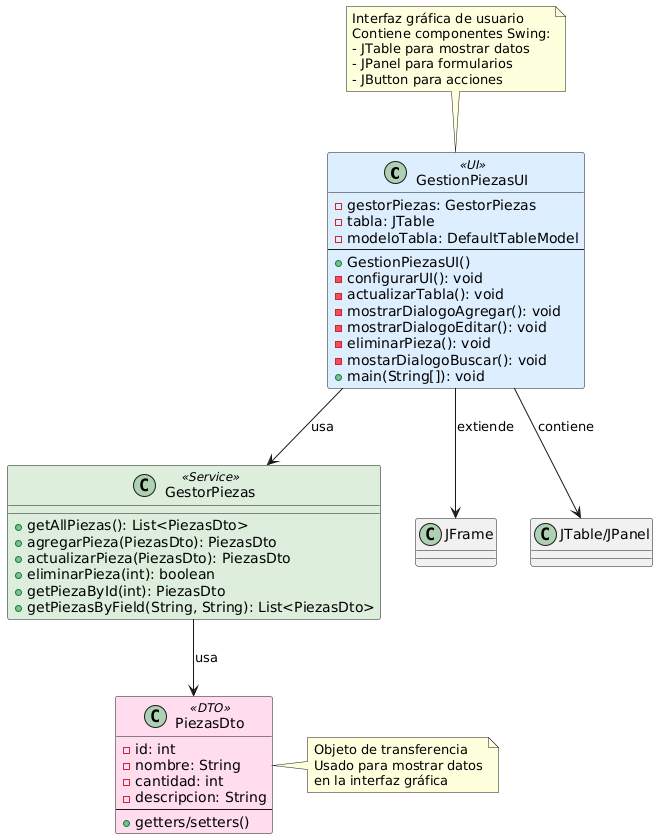
\includegraphics[width=0.5\textwidth]{imag/DiagramaFinalPL.png}
    \end{center}
     \item \textbf{Capa de Negocio:} Esta capa es la encargada de procesar la información. 
    En esta capa se realizaran todas las funciones del sistema a desarrollar.
    \newline
    
    \begin{center}
        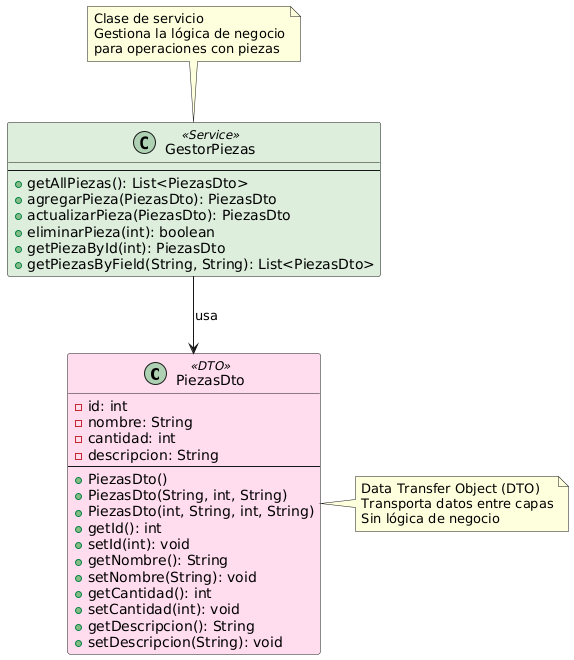
\includegraphics[width=0.5\textwidth]{imag/DiagramaFinalBL.png}
    \end{center}
    \item \textbf{Capa de Acceso a Datos:} Esta capa es la encargada de interactuar con la base de datos. 
    En esta capa se encuentran las consultas a la base de datos.\newline
    
    \begin{center}
        \includegraphics[width=0.5\textwidth]{imag/DiagramaFinalDAL.png}
    \end{center}
\end{itemize}

\subsection*{Vista de Casos de Uso}

    La vista de casos de uso se basa en los siguientes casos de uso:
    \begin{itemize}
        \item \textbf{Registrar Refacción:} Este caso de uso permite al usuario registrar una refacción.
        \item \textbf{Modificar Refacción:} Este caso de uso permite al usuario modificar una refacción.
        \item \textbf{Eliminar Refacción:} Este caso de uso permite al usuario eliminar una refacción.
        \item \textbf{Buscar Refacción:} Este caso de uso permite al usuario buscar una refacción.
    \end{itemize}

    \section*{Resumen de la Arquitectura}

\subsection*{Flujo Principal}
\begin{itemize}[leftmargin=*]
    \item \textbf{Capa de Presentación} (\texttt{GestionPiezasUI}):
    \begin{itemize}
        \item Interfaz gráfica Swing que captura interacciones del usuario
        \item Envía solicitudes al \texttt{GestorPiezas} (capa de negocio)
    \end{itemize}
    
    \item \textbf{Capa de Negocio} (\texttt{GestorPiezas}):
    \begin{itemize}
        \item Recibe DTOs (\texttt{PiezasDto}) de la UI
        \item Convierte DTOs a entidades (\texttt{Piezas}) para persistencia
        \item Delega operaciones CRUD al \texttt{PiezasDao}
    \end{itemize}
    
    \item \textbf{Capa de Datos}:
    \begin{itemize}
        \item \texttt{PiezasDao} implementa \texttt{EntityDao} para operaciones SQL
        \item Utiliza \texttt{DbConnection} para gestionar conexiones JDBC
        \item Persiste/recupera entidades \texttt{Piezas} en la base de datos
    \end{itemize}
\end{itemize}

\subsection*{Componentes Clave}
\begin{table}[h]
\centering
\begin{tabular}{|l|l|}
\hline
\textbf{Componente} & \textbf{Función} \\ \hline
\texttt{PiezasDto} & Transporte de datos entre capas (sin lógica) \\ \hline
\texttt{PiezasDao} & Implementa CRUD usando el patrón DAO \\ \hline
\texttt{Piezas} & Entidad que mapea la tabla de base de datos \\ \hline
\texttt{EntityDao} & Interfaz genérica para operaciones de persistencia \\ \hline
\texttt{DbConnection} & Gestiona conexiones JDBC con parámetros de configuración \\ \hline
\end{tabular}
\end{table}

\subsection*{Relaciones Críticas}
\begin{itemize}[leftmargin=*]
    \item \textbf{Dependecias: }
    \begin{itemize}
        \item UI $\rightarrow$ Gestor: La interfaz depende del gestor para lógica de negocio
        \item Gestor $\rightarrow$ (DAO + DTO): Coordina transformación y persistencia
        \item DAO $\rightarrow$ (Entidad + BD): Opera sobre la base de datos
    \end{itemize}
    
    \item \textbf{Conversión}: Transformación bidireccional entre \texttt{PiezasDto} (capa BL) y \texttt{Piezas} (capa DAL)
\end{itemize}

\subsection*{Patrones de Diseño}
\begin{description}
    \item[DTO (Data Transfer Object):] Separa la estructura de datos de la lógica de negocio
    \item[DAO (Data Access Object):] Abstracce el acceso a la base de datos
    \item[Separación de Capas:] Arquitectura en 3 niveles (UI, BL, DAL) con responsabilidades claras
\end{description}

\begin{figure}[h]
\centering
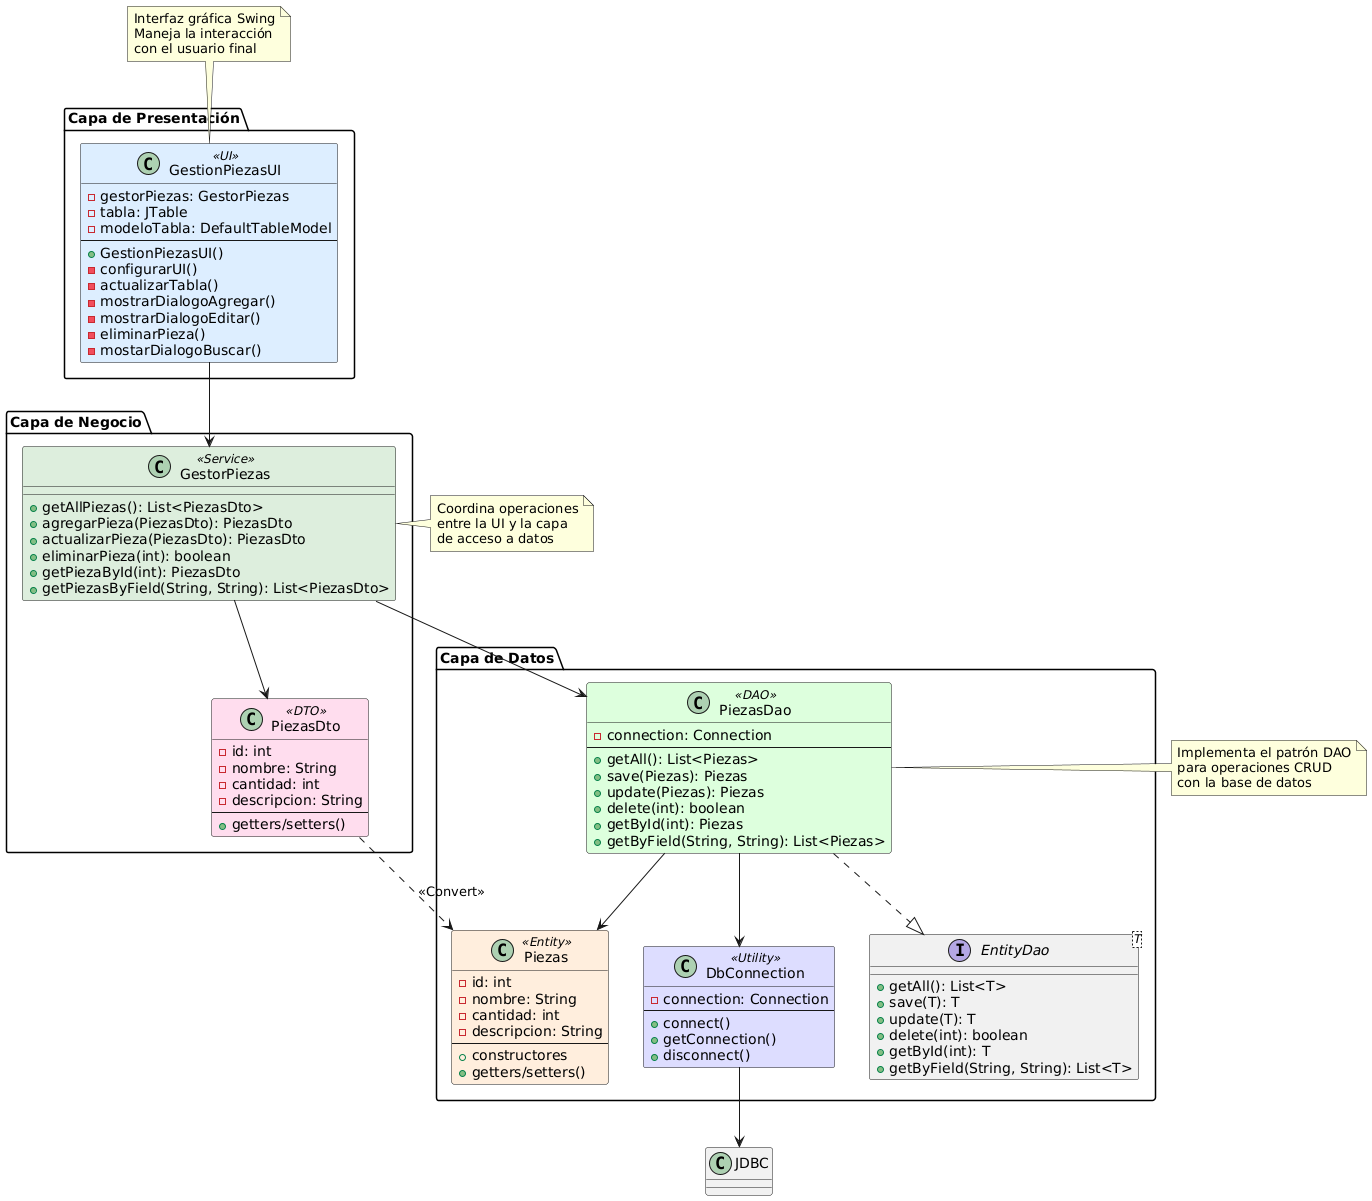
\includegraphics[width=0.9\textwidth]{imag/DiagramaFinalUML.png}

\end{figure}

